\documentclass[12pt]{article}


\usepackage[a4paper,top=3cm,bottom=2.5cm,left=3cm,right=4cm,marginparwidth=1.75cm]{geometry}
\usepackage{tgtermes} % times font

\linespread{1.25}
\usepackage{float}
\usepackage{hyperref}
\usepackage{graphicx}
\usepackage[pagetracker,notes,backend=biber]{biblatex-chicago}

\bibliography{main}
\begin{document}

\section{Alkoholkonsum in Baden Württemberg}



\subsection{Im zeitlichen Verlauf}
Schon im alten Griechenland wird in vielen Erzählungen über Saufgelage berichtet (TODO Quelle), damals war der Alkohol im Alltag allerdings verpönt (TODO Quelle). Erst seit dem Mittelarlter spielt Alkohol eine große Rolle in Europa. Ab dem ?? Jahrhundert wird er als ein wichtiger Teil der Ernährung von allen Altersgruppen mit etwa 3 Litern täglich Konsumiert (TODO Quelle). Man muss aber beachten, dass die Art dies Alkohols, die damals konsumiert wurde stark von heute abweicht. Ein großer Teil des Alkohols wurde z.B. in Form von Biersuppen konsumiert (TODO Quelle), bei deren Kochvorgang allerdings der Alkoholgehalt stark sank (TODO Quelle). Zu Beginn des 17. Jahrhunderts verbreiteten sich neue Genussmittel wie Kaffee, Kakao und Zucker in Europa, was zu einem starken Abfall des Alkoholkonsums führte (TODO Quelle). 

\subsection{Im Vergleich zu anderen Bundesländern}
Viele haben das Vorurteil, dass zwischen dem Trinkverhalten in den nördlichen und den südlichen Bundesländern in Deutschland ein großes Gefälle besteht. Ein Beispiel dafür ist das bayrische Oktoberfest, bei dem enorme Mengen an Alkohol konsumiert werden. Es wird auch als das größte Drogenfestival in Deutschland bezeichnet (TODO Quelle). Die Wissenschaft ist sich allerdings uneinig ob dieses Vorurteil wirklich zutrifft. Es gibt Studien die behaupten, dass es durchaus ein Gefälle zwischen dem Trinkverhalten im Norden und im Süden Deutschlands gibt \autocite{meyer_regionale_1998}. Eine andere Studie behauptet wiederum, dass diese Differenzen nur durch falsche Datenerhebung hervorgerufen werden \autocite{kraus_einfluss_2001}. Um diese Behauptungen genauer zu analysieren haben wir die Methoden dieser Studien untersucht: \\
Die Nord- und Südcluster wurden anhand von vergleichbaren Konsummustern definiert. In den südlichen Bundesländern wird mehr Bier getrunken, während im Norden mehr Wein und Spirituosen getrunken werden. Zum Südcluster gehören Nordrhein-Westfalen, Hessen, Rheinland-Pfalz, Saarland, Baden-Württemberg und Bayern und der Nordcluster besteht aus Niedersachsen, Hamburg, Schleswig-Holstein, Mecklenburg-Vorpommern, Brandenburg, Berlin, Sachsen, Sachsen-Anhalt und Thüringen. Bremen würde vom Konsummuster eher in den Südcluster passen und stellt daher eine Ausnahme dar. Trotz dieser unterdurchschnittlichen Konsummuster können bei der konsumierten Menge von Reinalkohol und bei der Prävalenz von riskantem Konsum keine signifikanten Unterschiede zwischen den Nördlichen und den Südlichen Bundesländern festgestellt werden. \autocite{kraus_einfluss_2001}.\\
Dieses Ergebnis wurde mit einer Analyse der Bundesstudien zum Konsum psychotischer Substanzen 1995 und 1997 erzielt \autocite{kraus_einfluss_2001}. Die von Meyer et al. \autocite{meyer_regionale_1998} vorgenommene Sekundäranalyse der Gesundheitssurvey Ost-West kommt allerdings zu dem Ergebnis, dass es signifikante Unterschiede in der Konsumierten Menge an Reinalkohol und der prävalenz von Riskantem Konsum zwischen Nord- und Süddeutschland gibt. Diese Ergebnisse wurden aber vermutlich dadurch verfälscht, dass die Angabe der Alkoholmenge pro Tag als Alkoholmenge pro Trinktag interpretiert wurde \autocite{kraus_einfluss_2001}. Daher sind die Ergebnisse dieser Studie vermutlich nicht aussagekräftig und wir können davon ausgehen, dass es zwischen Nord- und Süddeutschland keine siginifikanten Unterschiede in Trinkmenge und prävalenz für riskanten Alkoholkonsum gibt.

Wenn man allerdings die einzelnen Bundesländer genauer betrachtet fällt auf, dass in Bayern tatsächlich überdurchschnittlich viel Alkohol konsumiert wird \autocite{kraus_einfluss_2001}. In Baden Württemberg wird allerdings durchschnittlich relativ wenig Alkohol pro Tag getrunken. Auch der riskante Alkoholkonsum ist relativ gering. Da wir uns in unserer Seminararbeit hauptsächlich auf den Alkoholkonsum von Jugendlichen fokussieren wollen wäre eine Statistik zum durchschnittlichen Alkoholkonsum von Jugendlichen in den verschiedenen Bundesländern natürlich interessant. Bei unserer Recherche haben wir eine solche spezifische Statistik allerdings nicht gefunden. 

Um aber trotzdem eine Aussage über den Alkoholkonsum von Jugendlichen in Deutschland zu treffen, haben wir die Daten auf der Plattform GENESIS (Gemeinsames Neues Statistisches Informations-System) \autocite{noauthor_statistisches_nodate} verwendet. Auf GENESIS findet sich ein breit  gefächertes Datenangebot von den statistischen Landesämtern und dem Statistischen Bundesamt. Dieses enthält u.a. einen Datensatz mit dem Bundesland, Alter, Geschlecht und der Hauptdiagnose aller Krankenhauspatienten in Deutschland \autocite{noauthor_genesis_nodate}. Aus dieser Statistik haben wir alle Krankenhausaufenthalte von Jugendlichen bis 19 Jahren, die aufgrund von einer Alkoholintoxikation (Diagnose ICD-10 F10.0 \autocite{noauthor_icd-10-code_nodate}) im Krankenhaus waren extrahiert. In der folgenden Grafik sieht man diese im Durchschnitt pro 100.000 Einwohner des jeweiligen Bundeslandes über die letzten 15 Jahre aufgelistet.

\begin{figure}[H]
    \centering
    \includegraphics[scale=.7]{"assets/Alkohol_Bundesländer_avg_15_Jahre.png"}
    \caption{Alkoholbedingte Krankenhausaufenthalte von Jugendlichen in Abhängigkeit des Bundeslandes}
    \label{fig:Krankenhausaufenthalte_1}
\end{figure}

Für die Bevölkerungsanzahlen zur Normalisierung der Statistik wurde die Bevölkerung des jeweiligen Bundeslandes zum jeweiligen Zeitpunkt verwendet \autocite{noauthor_statistisches_2024}. Die Werte wurden mit Python berechnet und die Grafik wurde mit der Python Bibliothek Matplotlib \autocite{noauthor_matplotlib_nodate} erstellt. 

Es fällt auf, dass die Werte für kleine Bundesländer (Saarland, Hamburg und Berlin) stark abweichen. Das könnte an den geringen Fallzahlen liegen, die dann zu Extremwerten führen. Die absoluten Fallzahlen schwanken zum Beispiel im Saarland über die Jahre von 200 bis knapp 400. Ein weiterer wichtiger Aspekt, der bei der Analyse dieser Daten beachtet werden muss, ist der Länderaustausch von Patienten. Das Bundesland, in dem ein Patient behandelt wird, muss nicht mit dem Wohnort des Patienten übereinstimmen. Das kann aufgrund der Normalisierung der Daten zu einer Verfälschung der Ergebnisse führen. Auf GENESIS ist auch eine Statistik verfügbar, die statt dem Ort des Krankenhauses den Wohnort der Patienten angibt \autocite{noauthor_genesis_nodate-1}.

\begin{figure}[H]
    \centering
    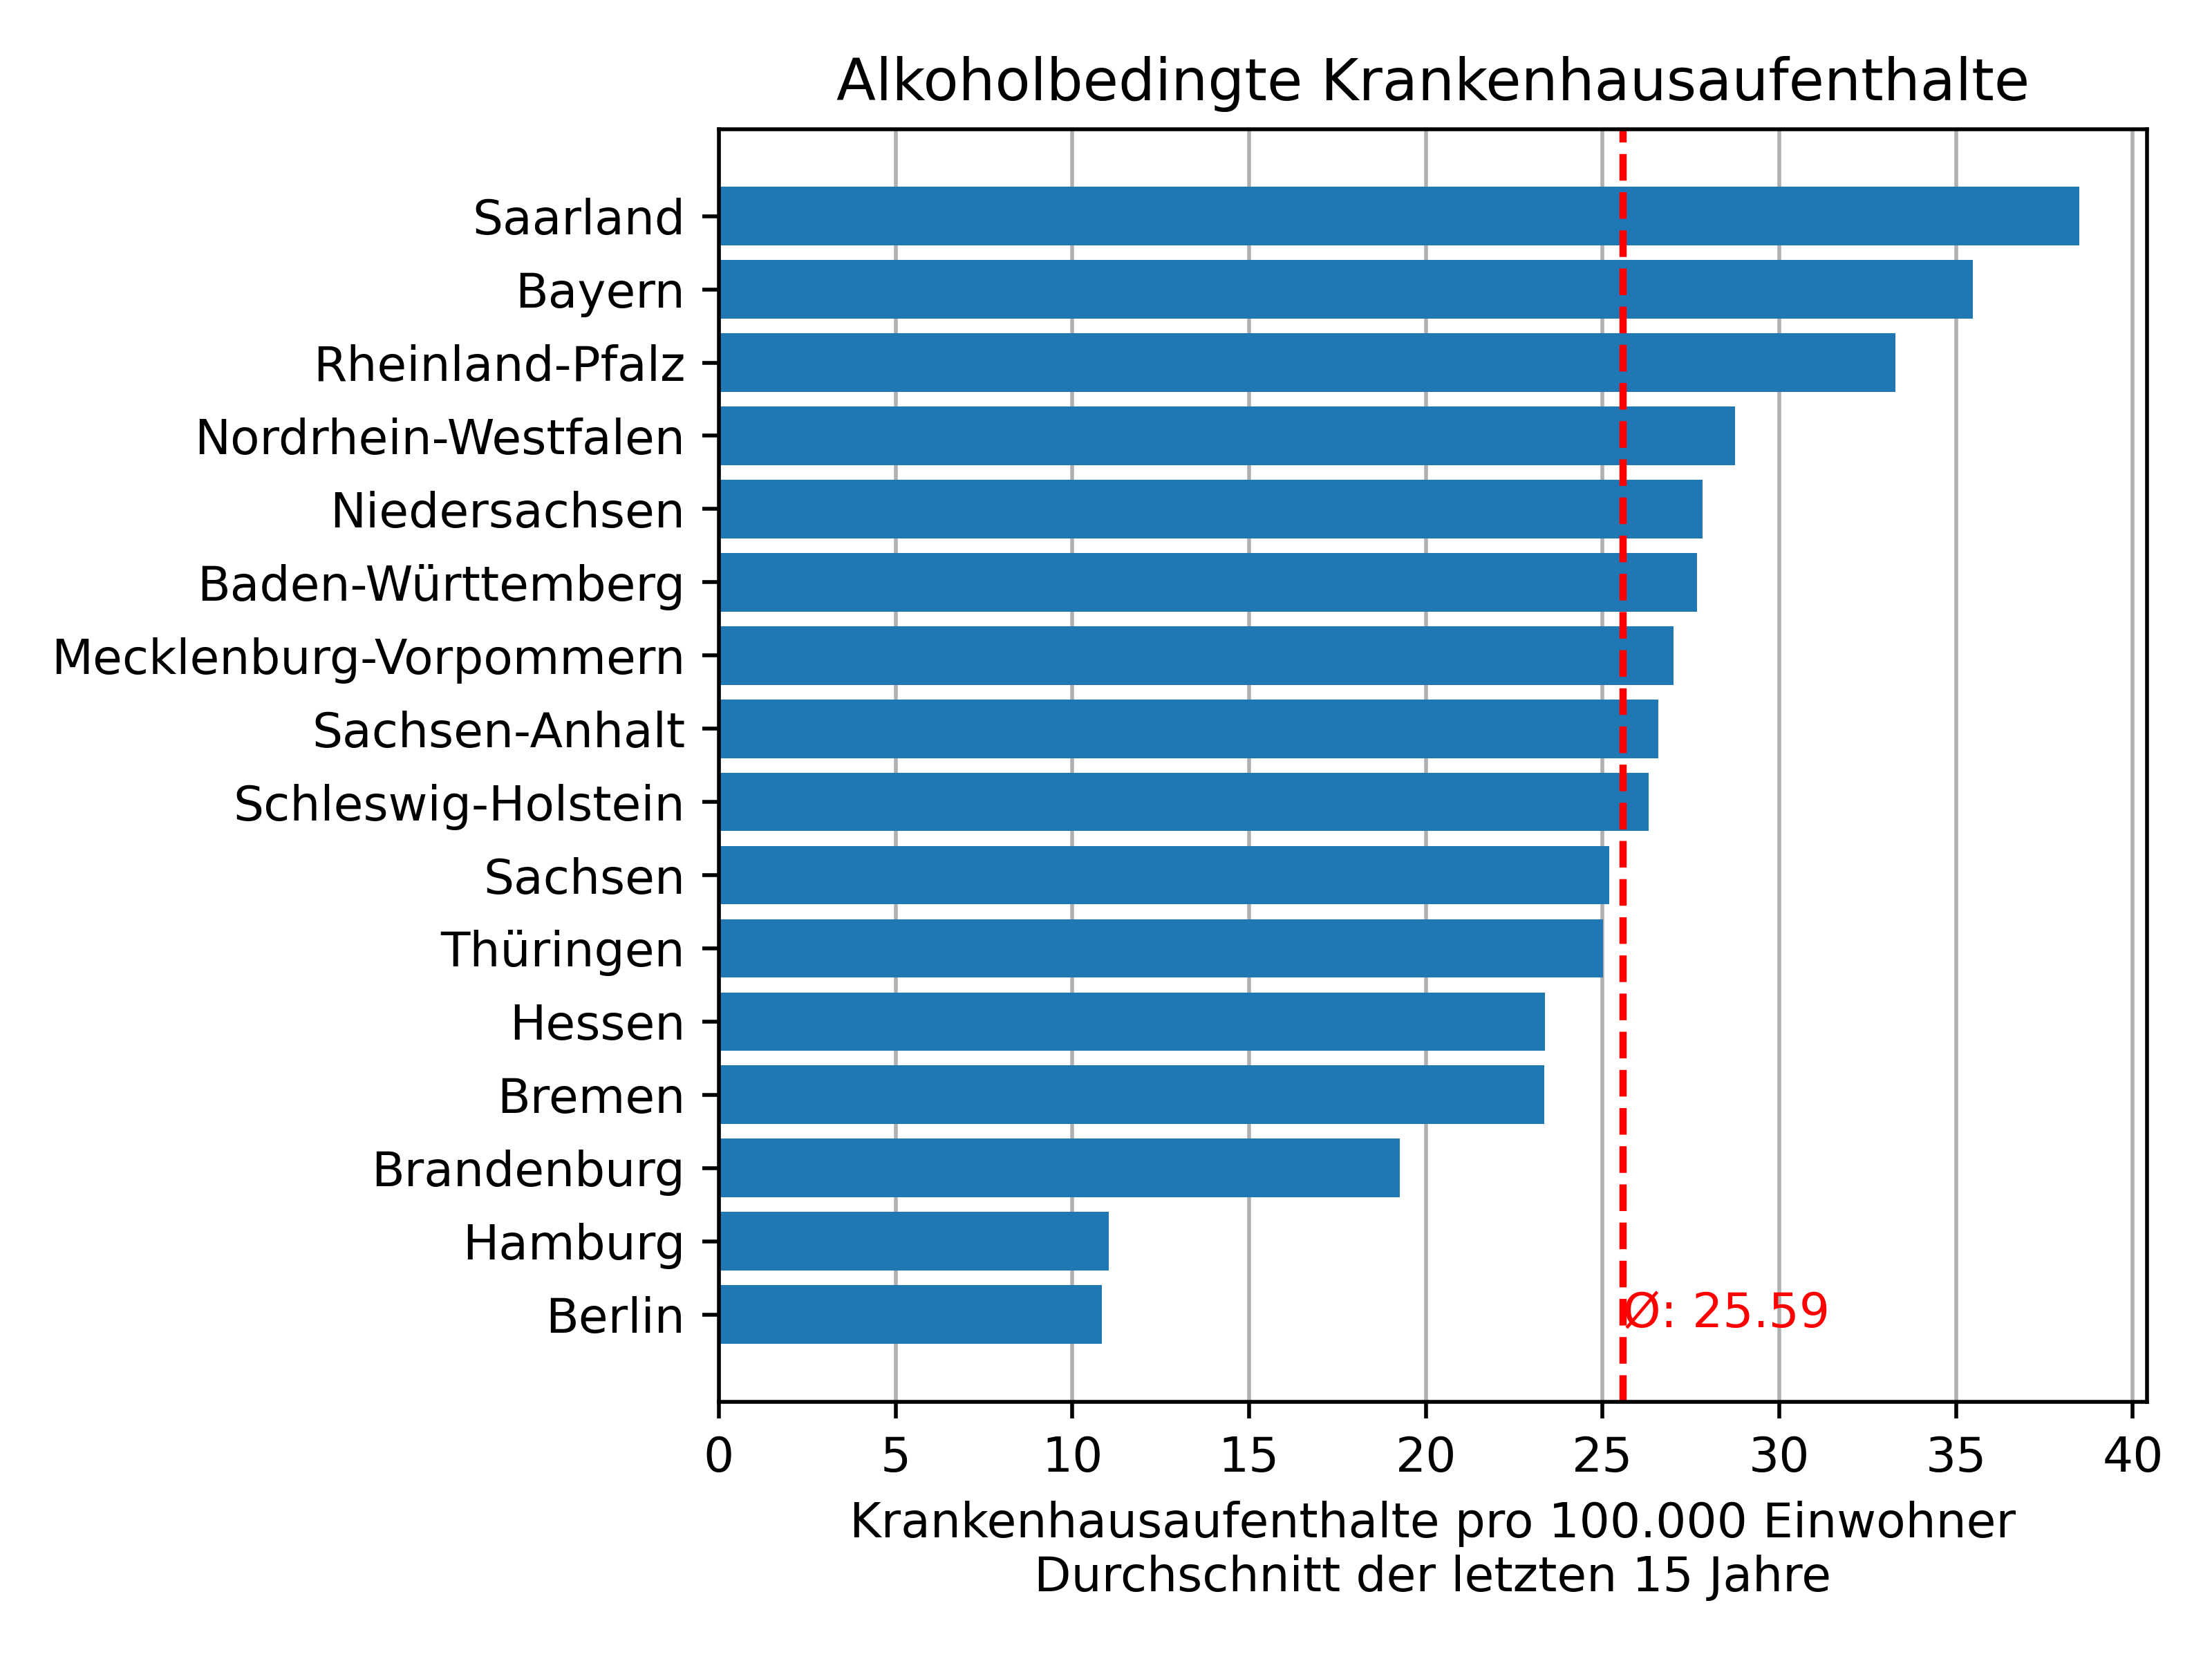
\includegraphics[scale=.7]{"assets/Alkohol_Wohnort_avg_15_Jahre.png"}
    \caption{Alkoholbedingte Krankenhausaufenthalte von Jugendlichen in Abhängigkeit des Wohnortes}
    \label{fig:Krankenhausaufenthalte_2}
\end{figure}

Grafik \ref{fig:Krankenhausaufenthalte_2} wurde mit den gleichen Methoden wie Grafik \ref{fig:Krankenhausaufenthalte_1} erstellt. Patienten deren Wohnort unbekannt ist und Patienten, die aus dem Ausland kommen wurden ignoriert. 
Die Werte für die meisten größeren Bundesländer sind nahezu gleich geblieben, da dort der Anteil der Patienten, die in einem anderen Bundesland behandelt wurden im Vergleich zu den Patienten, die in ihrem Heimatbundesland behandelt wurden sehr klein ist. Die Werte der kleineren Bundesländer (Hamburg, Berlin, Bremen und Saarland) sind dagegen stärker gesunken, vor allem bei Bremen. Das könnte daran liegen, dass ein Teil der Patienten, die zum Beispiel in einem Krankenhaus in Bremen behandelt wurden aus dem umliegenden Niedersachsen kommen. Dass die hohen Werte im Saarland kein Fehler in der Statistik sind, sondern ein reales Problem darstellen zeigt sich auch in diesem Artikel \autocite{noauthor_saarland_nodate}, der das Problem des Alkoholmissbrauchs von Jugendlichen im Saarland beschreibt. 
\\\\\\
Grafik \ref{fig:Krankenhausaufenthalte_1} und Grafik \ref{fig:Krankenhausaufenthalte_2} stellen den Durchschnitt der alkoholbedingten Krankenhausaufenthalte über die letzten 15 Jahre dar. Die folgende Grafik beschäftigt sich dagegen mit dem Zeitlichen Verlauf der alkoholbedingten Krankenhausaufenthalte in Baden-Württemberg und in Deutschland von 2000 bis 2022.
\begin{figure}[H]
    \centering
    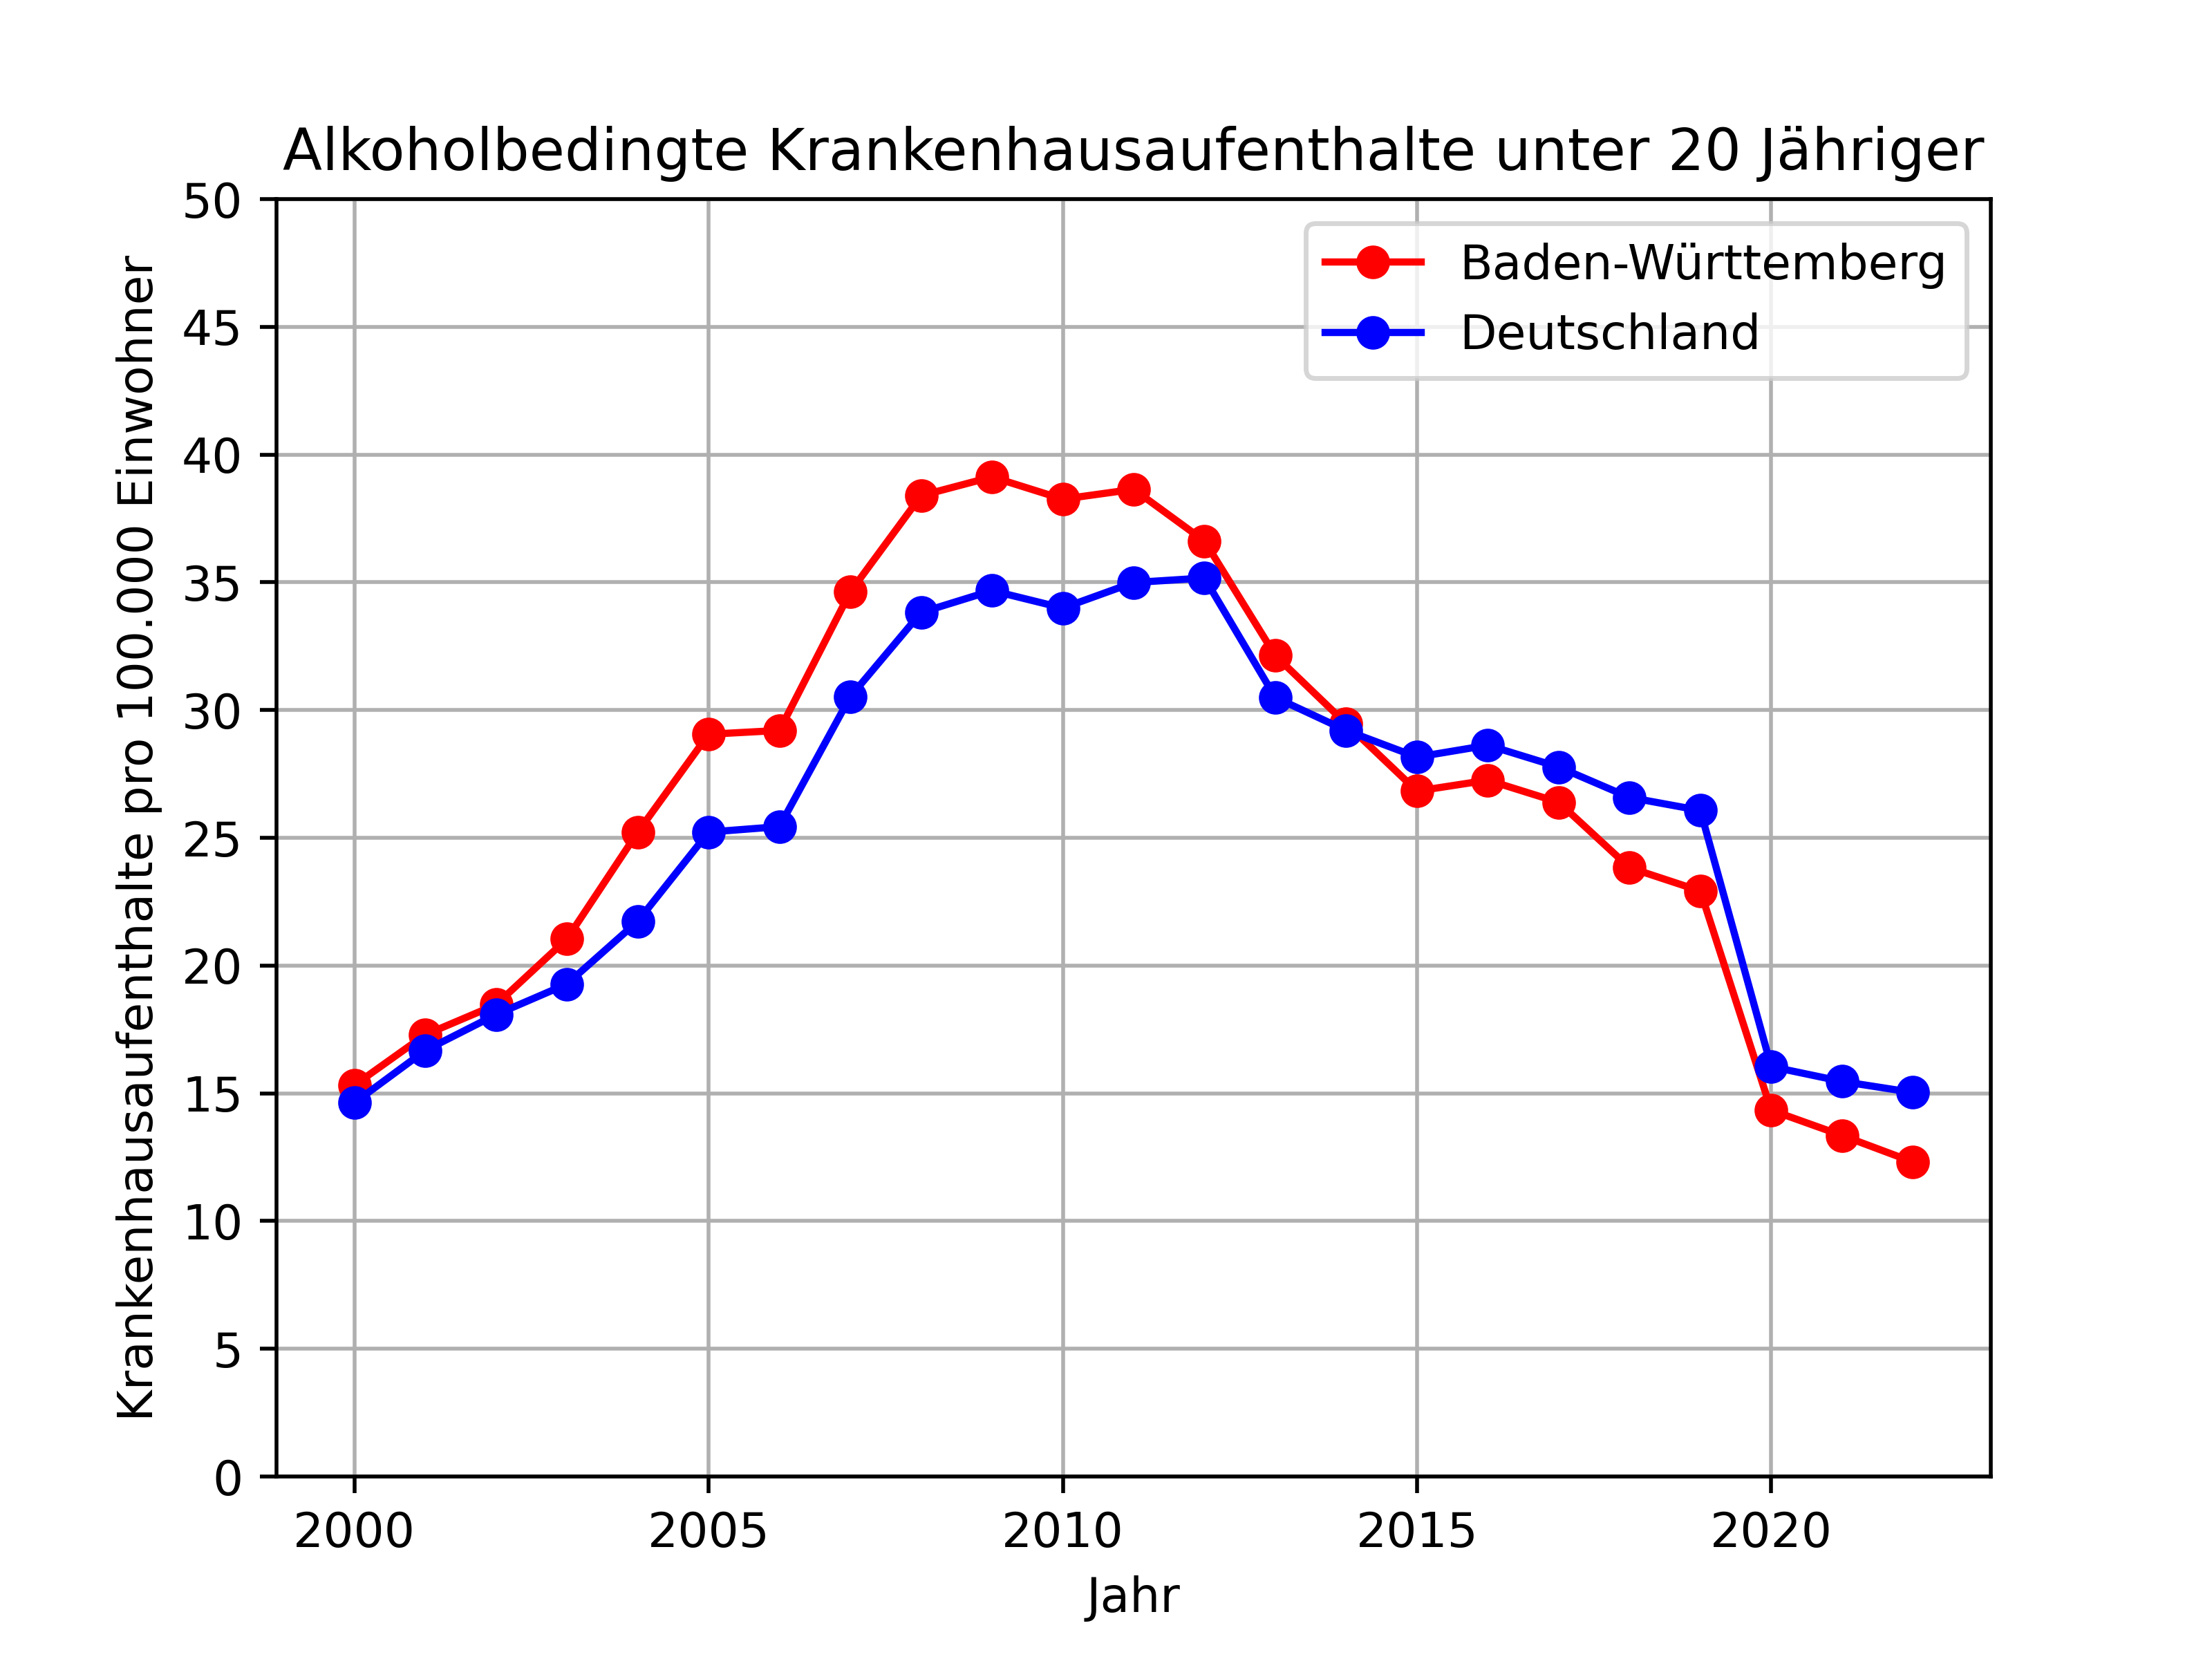
\includegraphics[scale=.7]{"assets/Alkohol_BW_Ges.png"}
    \caption{Alkoholbedingte Krankenhausaufenthalte von Jugendlichen von 2000 bis 2022}
    \label{fig:Krankenhausaufenthalte_3}
\end{figure}
Diese Grafik wurde ebenfalls mit den oben genannten Methoden erstellt.
Man sieht, dass sich die Verläufe von Baden-Baden Württemberg und Deutschland stark ähneln. Sie erreichen bis 2010 Höchstwerte und fallen bis 2019 auf ein Niveau von ca. 25 Krankenhausaufenthalte pro 100.000 Einwohner ab. Auch der Einfluss der Corona-Pandemie auf diesen Verlauf ist sehr gut zu erkennen, die Werte aus den Jahren 2020, 2021 und 2022 sind deutlich geringer als die der Jahre davor. Sogar die Tagesschau berichtet von derartigen Effekten \autocite{tagesschaude_weniger_nodate}.

Insgesamt kann man sagen, dass man auch an der Krankenhausstatistik sieht, dass der riskante Alkoholkonsum bei Jugendlichen in Baden-Württemberg von Jugendlichen nur geringfügig höher als der Bundesdurchschnitt ist.

\section{Eigene Umfrage}
Neben den vorherigen allgemeinen Auswertungen fanden wir es auch interessant, uns ein Bild von unserem eigenen Umfeld zu machen. Dafür haben wir über eine Iserv Umfrage über den Zeitraum von einer Woche alle Schüler der Klasse 10 sowie der Jahrgangsstufen 1 und 2.
\subsection{Auswertung}
Insgesamt haben 101 der 129 Schüler an der Umfrage teilgenommen, was einer Beteiligung von ungefähr 78 Prozent entspricht.
31 Stimmen sind von der Jahrgangsstufe 2, somit machen rund 30 Prozent aller Beteiligten aus. Am meisten teilgenommen haben die Schüler der Jahrgangsstufe 1. Hier haben sich 40 Schüler (39,6\%) die Zeit genommen, um die Fragen zu beantworten. Rein von der Anzahl der Teilnehmer nahmen am wenigsten Schüler der Klasse 10 teil. Von Ihnen haben 30 Schüler an der Umfrage teilgenommen. 
Jedoch muss man berücksichtigen, dass in der Klassenstufe 10 deutlich weniger Schüler sind als in den anderen Stufen. Somit ist der prozentuale Anteil der teilnehmenden Schüler in Klasse 10 mit 77\% wiederum am zweithöchsten nach der Jahrgangsstufe 1 (83\% aller Schüler in dieser Stufe). Die Jahrgangsstufe 2 hatte sich mit 73\% dennoch ebenfalls sehr gut an der Umfrage beteiligt.\\
Für uns sehr passend ist die ausgeglichene Beteiligung von männlichen und weiblichen Schülerinnen und Schüler, da es uns ermöglicht, die Resultate auf beide Geschlechter zu beziehen. 50 Schüler stehen in der Umfrage 49 Schülerinnen gegenüber, während lediglich 2 keine Angabe zu ihrem Geschlecht geben wollten. 
Vor dem Absenden der Umfrage haben wir uns vorgestellt, dass die meisten zwischen 14 und 15 das erste Mal Alkohol getrunken haben und diese Vermutung wurde letztendlich auch bestätigt. Über die Hälfte haben in diesem Zeitraum ihren ersten Kontakt zu Alkohol gehabt, wobei auch mit 13 relativ viele Schüler abgestimmt haben. Nur selten wurde bereits in jüngerem oder älterem Alter schon getrunken. Auch interessant, ganze 14 Leute haben noch nie Alkohol getrunken. \\
Bei der Frage, wie oft die Abgefragten aktuell noch trinken ist das Ergebnis ziemlich ausgeglichen. Zwischen ,,seltener als einmal im Monat“ und ,,häufiger als einmal in der Woche“ gibt es abgesehen von ,,mehrmals im Monat“ (24\%) kaum prozentuale Unterschiede (zwischen 11\% - 15\%). Von den ursprünglich 14 Schülern, welche noch nie Alkohol getrunken haben, trinken zwischenzeitlich neun Weitere keinen Alkohol mehr. Das bringt uns zu dem Schluss, dass manche einmal probiert und danach aber nichts mehr getrunken haben, wobei aber sicherlich auch welche dabei sind, die einfach so aufgehört haben. Dafür kann es verschiedene Anlässe geben, beispielsweise aus körperlichen oder gesundheitlichen Gründen wie einer entstandenen Allergie. 
Etwas überraschend fanden wir, dass Mischgetränke und purer Schnaps mit Abstand am beliebtesten waren. Knapp 70 Prozent trinken sehr gerne Mischgetränke, wenn sie auf einer Party sind und mit 39 Prozent trinken die Befragten am zweitmeisten Schnaps (Shots), was doch ein deutlicher Abstand zu Bier, welches am dritt-­beliebtesten ist (32\%). Etwas irritierend fanden wir allerdings, dass bei dieser Frage nur noch 22 Leute mit ,,keinen Alkohol“ abgestimmt haben. Wir konnten es uns nur so erklären, dass diese eine Person abgestimmt hat, welches Getränk sie früher am liebsten getrunken hat. \\
Unsere siebte Frage lautete ,,Wie viel trinkst du normalerweise an einem Tag?“. Interessiert hat uns dabei zu wissen, wie viel die Jugendlichen in unserem Alter an Getränken an einem Abend trinken. Wie bereits erwartet trinken die meisten zwischen drei und vier Getränke pro Party (23.76\%). Etwas darunter liegt die Auswahl zwischen fünf bis sechs (15.8\%) und ein bis zwei Getränken (10.9\%). Nur sehr selten trinken die Schüler mehr als sieben oder acht Getränke, wobei es natürlich ein paar Ausreißer gibt, die sogar mehr als 10 Getränke über den ganzen Abend trinken. Sehr verwunderlich ist allerdings, dass 37 Befragte angeben, sie trinken den ganzen Abend über nichts. Damit ist die Zahl der vorherigen Personen, die keinen Alkohol trinken innerhalb der letzten zwei Fragen um 14 Personen gestiegen. Das ist eine sehr große Anzahl, um von einem versehentlichen falschen abstimmen ausgehen zu können. \\
Natürlich war es für uns auch interessant zu sehen, zu welchem Anlass gerne getrunken wird, hierbei war eine Mehrfachauswahl möglich. Jede befragte Person, abgesehen von denen, die keinen Alkohol trinken, hat anagegeben, dass sie auf Partys und Geburtstagen Alkohol konsumieren. Weiter verbreitet ist der Konsum an Festen von Vereinen oder an Fasching. Die hälfte der Alkohol konsumierenden Schüler trinken auch, wenn sie bei der Verwandtschaft sind. Nur selten wird Alkohol allein oder am Feierabend getrunken (5-7\%). Auch die achte Frage ergibt erneut eine neue Anzahl an nicht Alkohol trinkenden Personen. 21 Schüler haben ,,Kein Alkohol“ angegeben. Zwar liegt der Wert wieder sehr eng bei den ersten Angaben, allerdings bringt dieser Wert ein anderes irritierendes Ergebnis mit sich. Mit einem Blick auf die Schüler, die angegeben haben, auf Partys und Geburtstagen Alkohol zu konsumieren (81 Schüler) und dann mit Blick auf diejenigen, die keinen Alkohol trinken (21) bemerkt man, dass insgesamt 102 Schüler abstimmen hätten müssen. Das Problem dabei ist, dass aber nur 101 Schüler an der Umfrage teilgenommen haben und es somit zu einer Überschneidung gekommen sein musste.\\ 
Im Hinblick auf Alkoholkonsum ist es immer wichtig zu schauen, trinkt man aus eigenem Antrieb oder wird man mehr dazu gedrängt, sei es Gruppenzwang, den man hat oder andere Menschen um einen herum, die versuchen dich dazu zu bringen, Alkohol zu trinken. Diese Frage haben wir uns auch gestellt und ebenfalls in unsere Umfrage mit aufgenommen. Erfreulich für uns war, dass 33 Schüler angaben, sie trinken immer aus eigenem Antrieb und 31 weitere, die immerhin meistens aus eigenem Antrieb trinken. Lediglich sieben Schüler werden manchmal zum Alkoholkonsum gedrängt und leider auch drei, die fast immer dazu gedrängt werden. Acht Schüler waren so ehrlich und haben angegeben, sie trinken immer aus eigenem Anlass, aber drängen andere auch dazu, etwas zu trinken. Auch hier variiert die Zahl der nicht Alkohol trinkenden Personen wieder und es sind nur noch 19.
Oft gibt es auch mal einen bestimmten Grund, wieso man an einem Tag keinen Alkohol trinken möchte. Bei unserer Umfrage haben die Teilnehmer bei Frage zehn als häufigsten Grund ,,keine Lust“ angegeben (64.4\%). Auch hier war wieder eine Mehrfachauswahl möglich. Andere Gründe, die viele angegeben haben, waren ein wichtiger Termin, beispielsweise ein Fußballspiel oder eine Klassenarbeit, am nächsten Tag (48.5\%) oder die Teilnahme am Straßenverkehr (43.6\%). Ebenfalls ungefähr gleich angegeben war der Grund, die anderen trinken auch nicht und es hat gesundheitliche Folgen (27-31\%). Die Anzahl der nicht Alkohol konsumierenden Schüler ist wieder auf 22 Schüler angestiegen, wobei dieser Wert bei dieser Frage etwas ungenau sein könnte, da zum Beispiel eine Person angegeben haben könnte, sie trinkt nicht aus gesundheitlichen Gründen und dann nicht mehr weitergelesen hat. \\
Jetzt hat sich nur noch die Frage gestellt, wie schätzen die Befragten ihren Konsum überhaupt selbst ein? Die meisten gehen davon aus, dass ihr Alkoholkonsum eher unterdurchschnittlich (25.7\%) oder durchschnittlich (28.7\%) ist. Knapp 17 Prozent geben ihren Alkoholkonsum zwischen den eben genannten Auswahlmöglichkeiten an. Wie es bereits zu erwarten war schätzen sich mit sieben und drei Schülern nur sehr wenige als etwas mehr und deutlich überdurchschnittlicher Alkoholkonsument ein. Die Zahl der nicht-Alkohol-Trinker ist erneut auf 19 Schüler gesunken. Auch im Hinblick auf gesundheitliche Auswirkungen werden sich in den drei Jahrgangsstufen kaum Sorgen gemacht. Ganze 38 Schüler haben angegeben, dass sie keine gesundheitlichen Auswirkungen von ihrem Alkoholkonsum haben und weitere 25 Prozent, dass sie auf lange Sicht keine gesundheitlichen Auswirkungen mit sich tragen, auch wenn es ihnen nur am nächsten Tag schlecht geht. Je stärker die gesundheitlichen Auswirkungen werden, umso weniger Schüler haben dafür abgestimmt. Lediglich noch 16 der Teilnehmer haben ihren Alkoholkonsum als Konsum mit geringen Auswirkungen auf die Gesundheit eingeschätzt, bei den moderaten Auswirkungen waren es dann nur noch zwei Schüler, die das angegeben haben. Als Konsum mit starken gesundheitlichen Auswirkungen hat keiner seinen Alkoholkonsum eingeschätzt. Bei dieser Frage haben wir wieder die Antwortmöglichkeit ,,kein Alkohol“ als Auswahl hinzugefügt, dafür haben 20 Schüler abgestimmt. 

\subsection{Fazit}
Im Rückblick auf unsere Umfrage sind wir sehr zufrieden damit, sie hat uns einen schönen Überblick über die Situation in unserem direkten Umfeld gegeben. Als allererstes war die Anzahl der teilnehmenden Schüler sehr gut. Mit einer Teilnahme von fast 80 Prozent aller Schüler sind wir sehr zufrieden. Ein Vorteil an der Teilnehmerzahl war für uns, dass wir beim Auswerten dadurch, dass es fast genau 100 Schüler insgesamt waren, sehr einfach zwischen der tatsächlichen Schülerzahl und dem prozentualen Anteil hin und her zu wechseln konnten, da dies immer dem ungefähr gleichen Wert entsprach. Auch mit der Auswahl der befragten Stufen sind wir am Ende zufrieden. Bevor die Umfrage gestartet haben, haben wir uns lang überlegt, ob wir nicht die neunten Klassen auch noch mitbefragen sollen, aber jetzt sind wir uns einig, dass es gut war, wie wir uns entschieden haben.\\
Teilweise haben sich unsere Vermutungen bestätigt. Ein sehr gutes Beispiel dafür sind die Angaben bei der letzten Frage, bei der unsere Vermutung vom Anfang bestätigt wurde, dass sich viele den Gefahren nicht bewusst sind. Aber es gab auch Überraschungen. Zu Beginn kam uns die deutlich höchste Beliebtheit an Mischgetränken und purem Schnaps gegenüber Bier und Sekt etwas überraschend vor. Mit längerem Überlegen wurde uns allerdings bewusst, dass der Grund dafür sein wird, dass Schnaps und Mischgetränke sowohl von Jungs als auf von Mädchen getrunken wird und Bier beziehungsweise Sekt nur von Jungs oder eben Mädchen und nur selten von beiden gleich gern getrunken wird.\\ 
Aber es war nicht nur positives an der Umfrage dabei und ein paar unpraktische Sachen gab es auch. Zum einen ist es unpraktisch, dass wir zwar sehen, wie viel aus welcher Jahrgangsstufe insgesamt abgestimmt haben, aber zum Beispiel beim aktuellen Konsum an einem Abend wiederum nicht sehen können aus welcher Jahrgangsstufe die Stimme gekommen ist. Ein weiteres Beispiel dafür ist die Vermutung. die wir am Anfang unseres Fazits getroffen haben. Wir haben vermutet die Beliebtheit an Schnaps liegt daran, dass bei Mädchen Bier und bei Jungs Sekt nicht so beliebt ist. Sicher belegen können wir es dadurch aber nicht. Wir haben uns zwar Gedanken gemacht, wie wir das ändern können, aber auf IServ Umfragen gibt es keine Möglichkeit dieses Problem zu lösen, ohne die Anonymität aufzuheben, aber das war keine Option. Zum anderen war es die große Schwankung der nicht Alkohol trinkenden Schülern, deren Anzahl dann am Ende von Frage zu Frage variiert hat. Natürlich gibt es da immer die paar Personen, die die Umfrage nicht ganz so ernst nehmen und sich einen Spaß daraus machen, einfach irgendwas bei der Umfrage anzukreuzen. Möglicherweise gab es aber auch Verständnisprobleme bei unseren Fragen. Es kann sein, dass ein paar Teilnehmer unsere Fragestellung nicht richtig oder anders verstanden haben und dadurch immer etwas Unterschiedliches abgestimmt haben. Dann könnten die Schwankungen den Ursprung bei uns selbst haben. Zusätzlich haben wir noch ein Problem beim Auswerten erkannt. Bei Frage sieben haben wir nach der Anzahl an Getränken gefragt. Sollte eine Person sehr gern nur Schnaps, also Shots trinken, steigt die Anzahl an Getränken sehr stark, obwohl es von der Menge weniger ist. Dies macht unsere siebte Frage ungenau und wir können sie nicht so gut nutzen.\\
TODO hier vlt no bissle umformulieren3
Eine paar Optimierung würden wir fürs nächste Mal auch gern treffen. Als erstes wollen wir die Fragen genauer und eindeutiger stellen, um unter anderem dem eben erwähnten Verständnisproblem vorzubeugen. Außerdem würden wir die Umfrage nächstes Mal gern länger laufen lassen und noch mehr Werbung machen, um noch mehr Schüler zu erreichen. 
Schlussendlich sind wir aber sehr zufrieden mit dem Ergebnis unserer Umfrage. 

\section{Problem}
Im ersten Teil haben wir ausführlich erfahren, dass Alkohol vor allem bei Jugendlichen und jungen Erwachsenen sehr schädlich ist. 
 %(TODO ggf bezug auf zeit)
In der obigen Analyse von verschiedenen Statistiken haben wir herausgefunden, dass es keine signifikanten Unterschiede zwischen der konsumierten Alkoholmenge in Nord- und Süddeutschland gibt. Insgesamt wird in Deutschland aber sehr viel Alkohol konsumiert, vor allem im weltweiten Vergleich. Laut der WHO wurden in Deutschland 2019 durchschnittlich 12.2 Liter Reinalkohol pro Kopf konsumiert, mehr als doppelt so viel wie der globale Durchschnitt von 5.5 Litern pro Kopf \autocite{noauthor_alcohol_nodate-1}. In Deutschland starben allein 2016 62.000 Menschen an allein auf Alkohol zurückzuführende Todesursachen \autocite{noauthor_alkoholkonsum_nodate}. Dafür bekommt Deutschland von der WHO einen YLL score von 3 von 5 \autocite{noauthor_alcohol-attributable_nodate }. Der YLL (years of life lost) score gibt die durchschnittliche Anzahl an Lebensjahren an, die durch einen vorzeitigen Tod durch eine Krankheit oder andere Todesursache im Vergleich zu der durchschnittlichen Lebenserwartung der Bevölkerung verloren wurde \autocite{martinez_reflection_2019}. Die WHO gibt mit diesem spezifischen score an, welcher Anteil des YLL scores der jeweiligen Bevölkerung durch Alkohol verursacht wurde. 1 ist hierbei der geringste Anteil, 5 der höchstmögliche.\\
Ein wichtiger Faktor für diesen hohen Alkoholkonsum ist vermutlich die unkritische Einstellung der Gesellschaft gegenüber Alkohol \autocite{noauthor_alkoholkonsum_nodate}. Das zeigt sich daran, dass weiten Kreisen der Gesellschaft alltäglicher Alkoholkonsum üblich ist, z.B. in Form von einem "Feierabendbier", einem "Verdauungsschnaps" oder einem "Gläschen Wein zur Tagesschau". Auch auf vielen Festen im süddeutschen Raum ist Alkoholkonsum ein wichtiger Aspekt. Das beste Beispiel hierfür ist natürlich das bayrische Oktoberfest, aber auch auf den meisten lokalen Festen wie z.B. Schützen oder dem Öchslefest ist der Alkohol für viele gar nicht wegzudenken. Diese unkritische Einstellung gegenüber von Alkohol fängt natürlich schon bei Jugendlichen an, auf denen auch der Fokus unserer Seminararbeit liegt. Auch in unserer Umfrage haben wir herausgefunden, dass viele Schüler bereits sehr früh mit dem Alkoholkonsum angefangen haben. Auffällig ist auch, dass 88\% aller befragten, die Alkohol konsumieren ihren Alkoholkonsum als durchschnittlich oder unterdurchschnittlich einschätzen und nur 12\% ihren Konsum selbst als überdurchschnittlich einschätzen. In der darauffolgenden Frage sollten die Schüler die Gesundheitlichen Auswirkungen ihres Alkoholkonsums selbst einschätzen. Alle Befragten haben dabei die Gesundheitlichen Auswirkungen höchstens als gering eingeschätzt, lediglich 2 Schüler waren der Meinung dass ihr Alkoholkonsum moderate gesundheitliche Auswirkungen hat. (TODO bezug auf gefahrenteil, ... der konsum der angegeben wurde hat durchaus gesundheitliche auswirkungen)\\

Auch in der obigen Analyse der Krankenhausstatistik haben wir herausgefunden, dass in Deutschland eine signifikante Anzahl an Jugendlichen aufgrund von einer Alkoholintoxikation im Krankenhaus behandelt werden muss. Die Anzahl der Jugendlichen, die große Mengen an Alkohol trinken, deswegen aber nicht im Krankenhaus behandelt werden müssen ist natürlich dementsprechend viel größer, was man auch an unserer Iserv Statistik erkennen kann. % TODO vlt bissle mehr hier
Daher beschäftigen wir uns im folgenden mit verschieden Methoden um Jugendliche vor den Gefahren des Alkohols zu beschützen. 

\subsection{Prävention}

\subsubsection{Empfehlungen des Gesundheitsministeriums}
Das Gesundheitsministerium hat eine Broschüre erstellen lassen, in der Empfehlungen für Eltern im Bezug auf den Alkoholkonsum ihrer Kinder zusammengefasst sind \autocite{kuhn_empfehlungen_nodate}. Die Broschüre richtet sich an Fachkräfte der Suchtprävention, die diese Regeln an Eltern weitergeben sollen. Die enthaltenen Empfehlungen basieren auf einer ausführlichen Literaturanalyse durch Experten. Ab Seite 16 finden sich konkrete Handlungsempfehlungen für Eltern:\\
Wichtig ist, dass Eltern sich gut über die Wirkung von Alkohol, aber auch über die gesetzlichen Bestimmungen informieren. Dadurch sollten die Eltern dann in der Lage sein die Fragen ihrer Kinder zu diesem Thema zu beantworten und diese zu informieren. Dabei sollten zwar die Gefahren und Risiken sachlich aufgezeigt, aber auf keinen Fall dramatisiert werden.\\
Auch die Vorbildfunktion der Eltern ist ein wichtiger Einflussfaktor. Sie sollten daher auf einen Alkoholkonsum achten, der ein gutes Vorbild darstellt.  

TODO studie zu prävention zotero

\subsection{Verbote}
Weitreichende Verbote sind für den Alkoholkonsum von jugendlichen in Deutschland keine wirksame und sinnvolle Lösung. Nehmen wir an, das Mindestalter für den Alkoholkonsum wird um zwei Jahre erhöht, d.h. Bier, Wein und Sekt dürften erst ab 18 Jahren konsumiert werden. Ein solches Verbot bräuchte einen großen Rückhalt in der Gesellschaft, da Jugendliche unter 18 Jahren sonst durch Eltern oder ältere Bekannte einfach an Alkohol gelangen könnten. Auch den erhöhten Reiz, den ein Verbot auf Jugendliche haben kann, darf man nicht außer Acht lassen \autocite{skala_jugend_2020}. 
Allein an unserer Iserv-Umfrage und an der Krankenhausstatistik kann man deutlich erkennen, dass ein solches Verbot nur einen geringen Effekt haben würde. Von den Schülern der Stufe 10, 11 und 12 die bereits einmal Alkohol getrunken haben haben nur 10\% mit 16 oder älter das erste mal Alkohol getrunken. 
% TODO satz nicht so scheiße formulieren 
TODO Quelle hier in den Empfehlungen für die Eltern, blau marktiert





TODO quelle empfehlungen für eltern vom Gesundheitsministerium sehr gut

TODO bei gefahren: Empfehlungen vom Gesundheitsministerium als quelle (in grün)

TODO werbung für alkohol
\printbibliography
\end{document}
